\section{Related Work}
\label{ch:related-work}

\epigraph{That men do not learn very much from the lessons of history is the most important of all the lessons that history has to teach.}{Aldous Huxley}

\subsection{Recommend System}
Francesco et al. systematically and comprehensively describe the recommendation system in the handbook for Recommender Systems \cite{ricci2011introduction}. A recommendation system is a software tool and technology used to provide suggestions and recommendations to users. The recommendations are designed to provide users with choices in various decision-making processes, such as which products to pick, which movies to watch, or what news to read. It turns out that the recommendation system can be used to solve the problem of user information overload, and has become one of the most powerful and popular tools in e-commerce. Corresponding to the recommendation system is search engine technology, various technologies for generating recommendations have been proposed, and in the past ten years, many recommendation systems have been successfully deployed in commercial environments.
\par The entire recommendation system can be regarded as a processing plant, inputting user and item data, outputting a list of items that the user may be interested in, and then taking the first several from the item list as the recommendation result to the user.
\par In this process, we need to do some filtering and sorting. When outputting results, it is best to let users know why this is recommended, so that the user's acceptance will be higher.
\par Through some mathematical algorithms, guess what users might like. The recommendation algorithms use some of the user's behavior and some mathematical algorithms to infer what the user might like.
\par The recommendation algorithm is performed by a machine. While it can process a large amount of information, it is not so humane. In the process of pushing recommendations to the user, the powerful processing energy of the machine can deal with much more information than humans.

\subsection{Explainable Recommendation}
\subsubsection{Definition}
Explainable Recommendation refers to the personalized recommendation algorithms that address the problem of why - they not only provide users with the recommendations, but also provide explanations to make the user or system designer aware of why such items are recommended. In this way, it helps to improve the effectiveness, effeciency, persuasiveness, and user satisfaction of recommendation systems. Yongfeng et al. first highlight the position of explainable recommendation in recommender system research by categorizing recommendation problems into the 5W, i.e., what, when, who, where, and why, in their survey \cite{zhang2018explainable}. 
\\
\\
\textbf{When:} time-aware recommendation \\
\textbf{What:} application-aware recommendation \\
\textbf{Who:} social recommendation \\
\textbf{Where:} location-based recommendation \\
\textbf{Why:} explainable recommendation \\
\par Research on the question about "Why" has created a new research area: explainable recommendation.
\par To make personalized recommendation models intuitively understandable, researchers have more and more turned to the study of Explainable Recommendation Models, where the recommendation algorithm not only provides a recommendation list as output, but also naturally works in an explainable way and provides explanations to accompany the recommendations \cite{mcauley2015image}.
\par There are many different display styles of explanations: Explanation based on Relevant Users or Items, Feature-based Explanation, Textual Sentence Explanations, Visual Image Explanations and Social Explanation. Explanation based on relevant users or items, which presents nearest-neighbor users or items as explanation, and the relevant users or items are provided by user-based or item-based collaborative filtering methods. In this thesis, we will use a Path Generate Algorithm based on nearest-neighbor to build the model of our explainable recommendation system.
\par Explanation based on relevant users or items, which presents nearest-neighbor users or items as explanation, and the relevant users or items are provided by user-based or item-based collaborative filtering methods. User-based and item-based collaborative filtering \cite{sarwar2001item}, \cite{cleger2012top} are two fundamental methods for personalized recommendation.
\par Feature-based explanation, which provides users with the item features that match with the target user?s interest profile as explanation.
\par We combine these two and build a hybrid explainable recommendation system that can handle both types of explainable recommendations simultaneously.

\subsubsection{Graph-based Models for Explanation}
Graphs can be used to represent user-user or user-item relationships in most cases. Various studies have assessed the efficacy of Graph-based Models for Explanation. Graph learning approaches such as graph-based propagation and graph clustering can be used to generate the explainable recommendations. Most research on modeling for explainable recommendation has been carried out in Graph-based model. He et al.\cite{he2015trirank} described a tripartite graph to model the user-item-aspect ternary relation for a top-N recommendation. They proposed TriRank, a common-used algorithm for ranking on tripartite graphs by regularizing and normalizing the fitting constraints and smoothness.
\par Based on the user-item bipartite graph for the explainable recommendation, Reinhard and his team \cite{heckel2017scalable} proposed to conduct over-lapping co-clustering, without using external information such as aspects. The users have similar interests and the items are of similar features in each co-cluster. 

\begin{figure}[h]
\caption{OC-uLaR algorithm example\cite{heckel2017scalable}}
\label{figure:2-1}
\centering
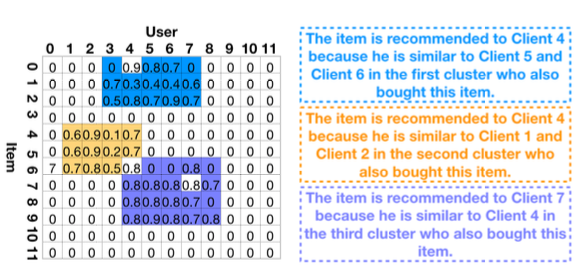
\includegraphics[width=0.8\textwidth]{oc_ular_algorithm}
\end{figure}

\subsection{Graph Neural Network Algorithm}
\subsubsection{GCN}
Graph Convolutional Network (GCN) can be used to build most of the large datasets we already have. For these models, the goal is then to learn a function of signals/features on a graph $ G=(\upsilon ,\varepsilon ) $.\\

\begin{figure}[h]
\caption{modularity-based clustering GCN}
\label{figure:2-2}
\centering
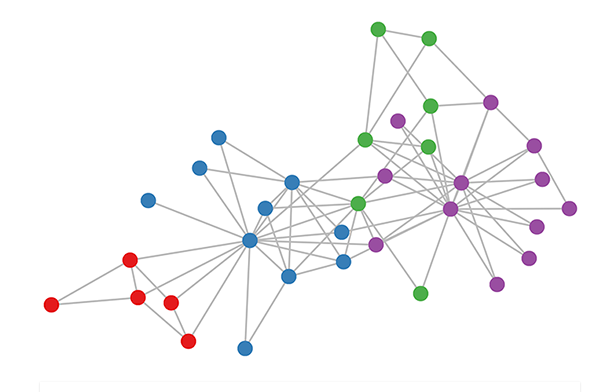
\includegraphics[width=1\textwidth]{gcn_algorithm}
\end{figure}

\begin{itemize}
\item[(i.)] A feature description $x_{i}$ for every node i; summarized in a N$\times$D feature matrix X (N: number of nodes, D: number of input features).
\item[(ii.)] A representative description of the graph structure in matrix form; typically in the form of an adjacency matrix A (or some function thereof).
and produces a node-level output Z (an N$\times$F feature matrix, where F is the number of output features per node). Graph-level outputs can be modeled by introducing some form of pooling operation. \cite{duvenaud2015convolutional}
\[
f(H^{l},A) = \sigma (AH^{(l)}W^{(l)});
\]
\end{itemize}
the above is a very simple form of a layer-wise propagation rule. Duvenaud and his team \cite{duvenaud2015convolutional} address two limitations of this simple model: 
\begin{itemize}
\item[(j.)] Multiplication with A means that, for every node, we sum up all the feature vectors of all neighboring nodes but not the node itself (unless there are self-loops in the graph).
\item[(jj.)] A  is typically not normalized and therefore the multiplication with A will completely change the scale of the feature vectors (we can understand that by looking at the eigenvalues of A).
They essentially describe a new propagation rule introduced in \cite{kipf2016semi}:
\[
f(H^{l},A) = \sigma (\hat{D}^{-\frac{1}{2}} \hat{A}\hat{D}^{-\frac{1}{2}}H^{ (l) }W^{ (l) }) ;
\]
\end{itemize}

\subsubsection{GraphSAGE}
It turns out that low-dimensional vector embeddings of nodes in large graphs are extremely useful as feature inputs for various prediction and graph analysis tasks. Hamilton and his team\cite{hamilton2017inductive}describe the embedding generation, or forward propagation algorithm , which assumes that the model has already been trained and that the parameters are fixed. In particular, they assume that they have learned the parameters of K aggregator functions. The key idea of the method GraphSAGE behind their approach is that they learn how to aggregate feature information from a node's local neighborhood. Specifically, they use Embedding generation (i.e., forward propagation) algorithm in algorithm \ref{algorithm:1}.
\par Our kernel recommend algorithm for generating path is conceptually inspired by a classic algorithm for testing graph isomorphism and GraphSAGE algorithm.
\\
\\
\\
\begin{algorithm}[H]
\SetAlgoLined
\textbf{Input:} Graph G($\nu$, $\varepsilon $); input features \{x$_{v}$, $ \forall $ v $ \in $ V\}; depth K; weight matrices W$ ^{k} $, $ \forall $k $ \in $ \{1, ..., K\}; non-linearity $ \sigma $; differentiable aggregator functions AGGREGATE$_{k}$, $ \forall $ k $ \in $ \{1, ..., K\}; neighborhood function N : v  $ \rightarrow $ 2$ ^{v} $  \\

\textbf{Output:} Vector representations z$_{v}$ for all $\nu$ $ \in $ V \\
h$_{v}^{0}$ $ \leftarrow \chi _{v},\forall v\in V $ \\
 \For{k = 1...}{
 \For{$ v\in V $}{
 $ h_{N_{(v)}}^{k}\leftarrow AGGREGATE_{k}(\{ h_{u}^{k-1},\forall u \in N(v) \}) ; $ \\
 $ h_{v}^{k} \leftarrow \sigma\left ( W^{k} \cdot CONCAT(h_{v}^{k-1},h_{N_{(v)}}^{k}) \right ) ; $ \\
 }
 $ h{_{v}}^{k} \leftarrow {h{_{v}}^{k} / \left \| h{_{v}}^{k} \right \|} _{2},\forall v \in \nu ; $ \\
 }
 $ z_{v} \leftarrow h_{v}^{k}, \forall v \in \nu $ \\
 \caption{GraphSAGE Embedding Generation Algorithm}
 \label{algorithm:1}
\end{algorithm}

\begin{figure}[h]
\caption{Visual illustration of the GraphSAGE sample and aggregate approach}
\label{figure:2-3}
\centering
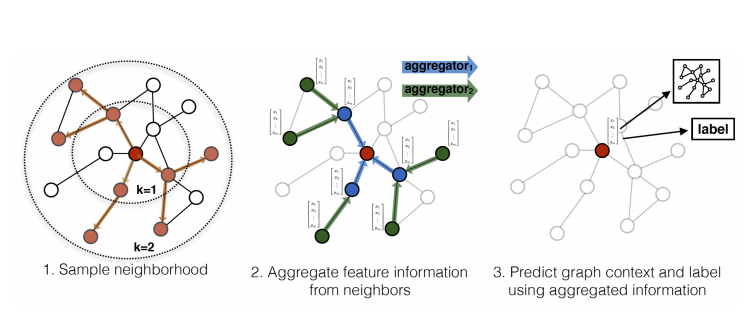
\includegraphics[width=1\textwidth]{GraphSAGE_algorithm}
\end{figure}

\cleardoublepage